\section{Evaluating the impact of synthetic rain}
\label{sec:impact_synth}


To study how vision algorithms perform under increasing amounts of rain, we leverage our rain synthesis pipeline and augment popular clear-weather datasets. Specifically, our PBR and GAN+PBR frameworks allow us to measure the performance of these algorithms in \emph{controlled} rain settings.

\subsection{Rain generation setup}
\label{sec:rain_setup}

We augment all three of the KITTI, Cityscapes, and nuScenes-clear datasets with PBR. 
We generate rainfall rates ranging from light to heavy storm $R = \{0, 5, 25, 50, 100, 200\}$~mm/hr. 
Only the nuScenes-clear dataset is augmented with GAN and GAN+PBR, since neither KITTI nor Cityscapes contain rainy images to train the GAN. 
Our PBR and GAN+PBR rain augmentation require some preparation as they rely on calibration, depth and camera motion. Our GAN and GAN+PBR rain augmentation require the training of a CycleGAN. These preparations are described below.

\paragraph{Calibration.} For the realistic physical simulator (sec.~\ref{sec:raindrop-position}) and the rain streaks photometric simulation (sec.~\ref{sec:photometry-rainstreak}), intrinsic and extrinsic calibration are used to replicate the imaging sensor. 
We used frame-wise or sequence-wise calibration for KITTI and nuScenes. 
In addition, we use 6mm focal and 2ms exposure for KITTI~\cite{Geiger2012CVPR,Geiger2013IJRR} and assumed 5ms exposure for nuScenes.
As Cityscapes does not provide calibration, we use intrinsic from the camera manufacturer with 5ms exposure and extrinsic is assumed similar to KITTI. 

\paragraph{Depth.} The scene geometry (pixel depth) is also required to model accurately the light-particle interaction and the fog optical extinction. 
We estimate KITTI depth maps from RGB+Lidar with~\cite{jaritz2018sparse}, and Cityscapes/nuScenes from monocular RGB with Monodepth~\cite{monodepth17,godard2019digging}.
While absolute depth is not required, we aim to avoid the critical artifacts along edges, and thus further align RGB with depth using guided filter~\cite{barron2016fast}. 

\paragraph{Camera motion.} We mimic the camera ego motion in the physical simulator to ensure realistic rain streak orientation on still images and preserve temporal consistency in sequences.
Ego speed is extracted from GPS data when provided (KITTI and nuScenes), or drawn uniformly in the $[0, 50]$~km/hr interval for Cityscapes semantics and in the $[0, 100]$~km/hr interval for KITTI object to reflect the urban and semi-urban scenarios, respectively.

\paragraph{CycleGAN.} A CycleGAN is trained for image-to-image rain translation on the train subsets of nuScenes-clear and nuScenes-rain (sec.~\ref{sec:real_data}). In order to make sure that no image is used to both train and evaluate the GAN simultaneously, we use the 4449 images from the nuScenes-clear(test) subset, resize them to $448\times256$, and perform image-to-image translation to generate GAN-augmented rain images. We dub this new set of images ``nuScenes-augment'' for clarity, and will also use this for the GAN+PBR rain augmentation. 

\begin{figure}
 \centering
 \subfloat[Object detection]{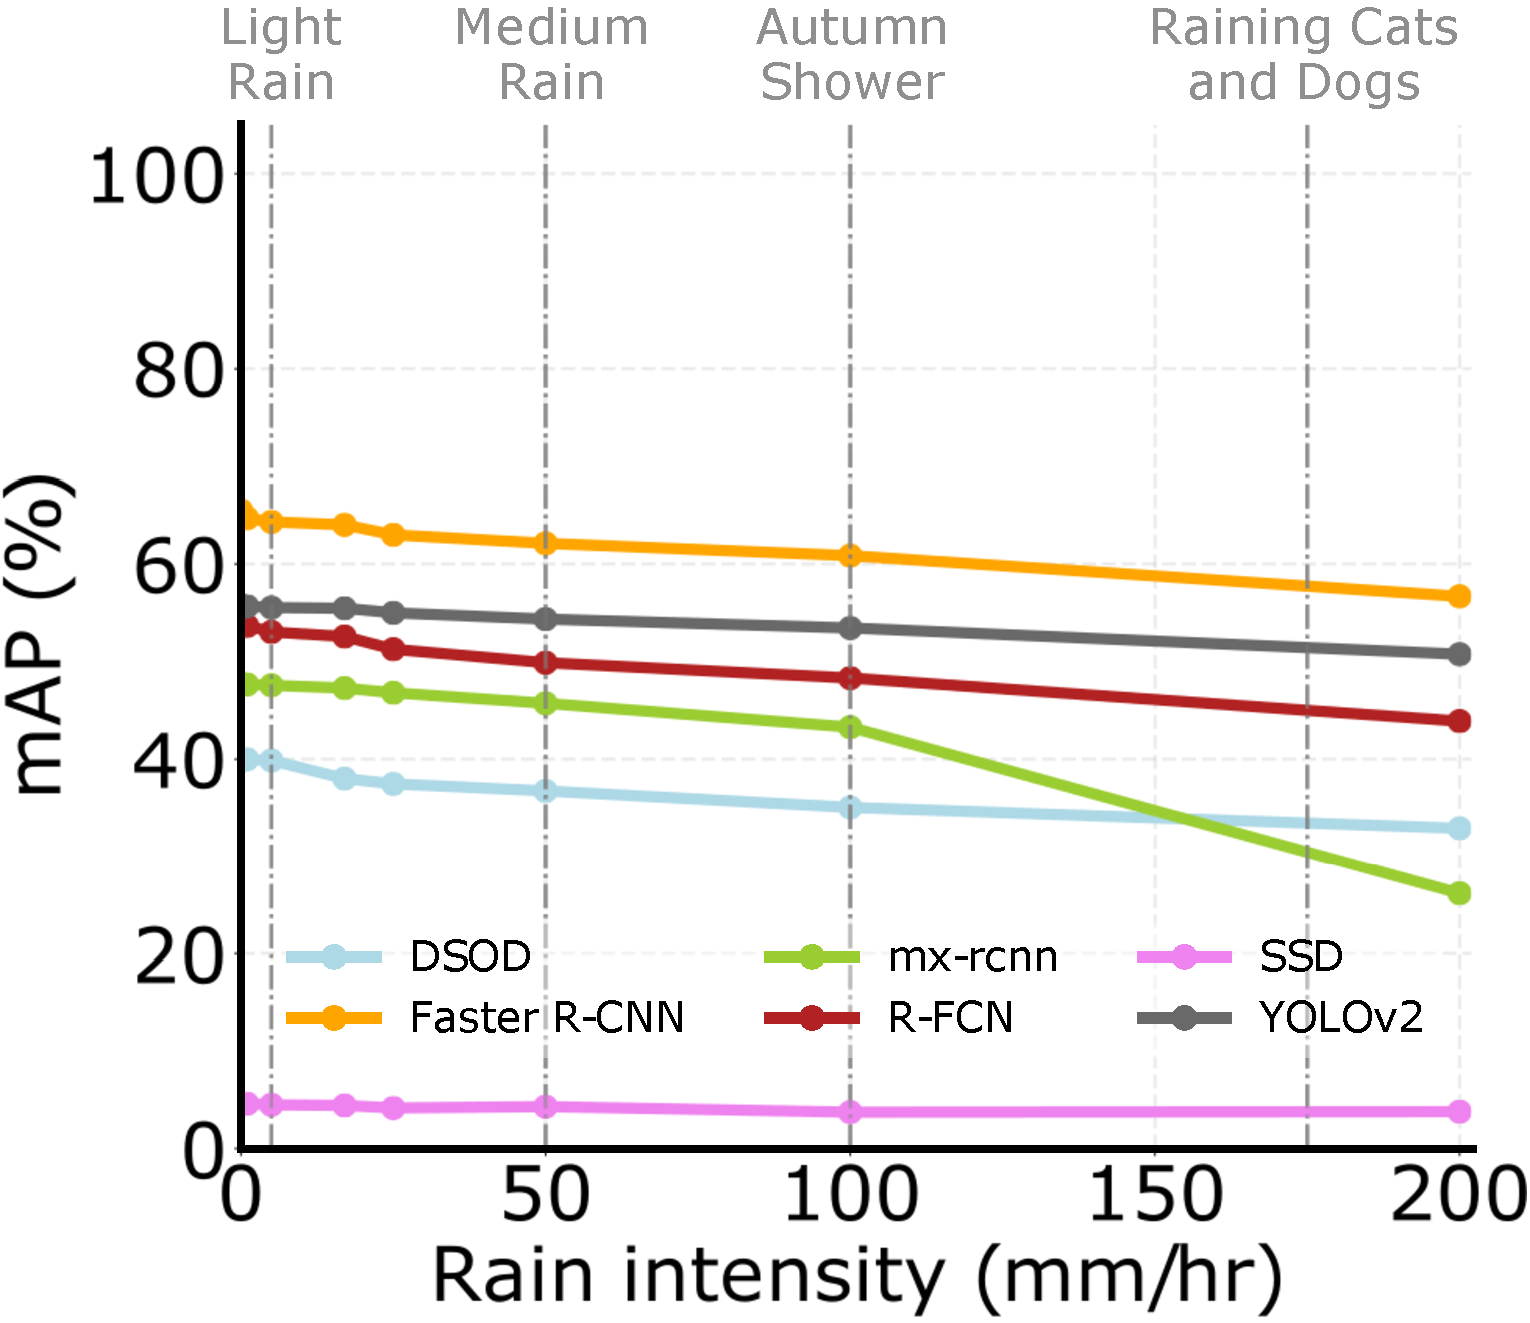
\includegraphics[width=0.485\linewidth]{figures/plots/obj_detection_perf_rain.pdf}\label{fig:algo_obj_detect_perf}}
 \subfloat[Semantic segmentation]{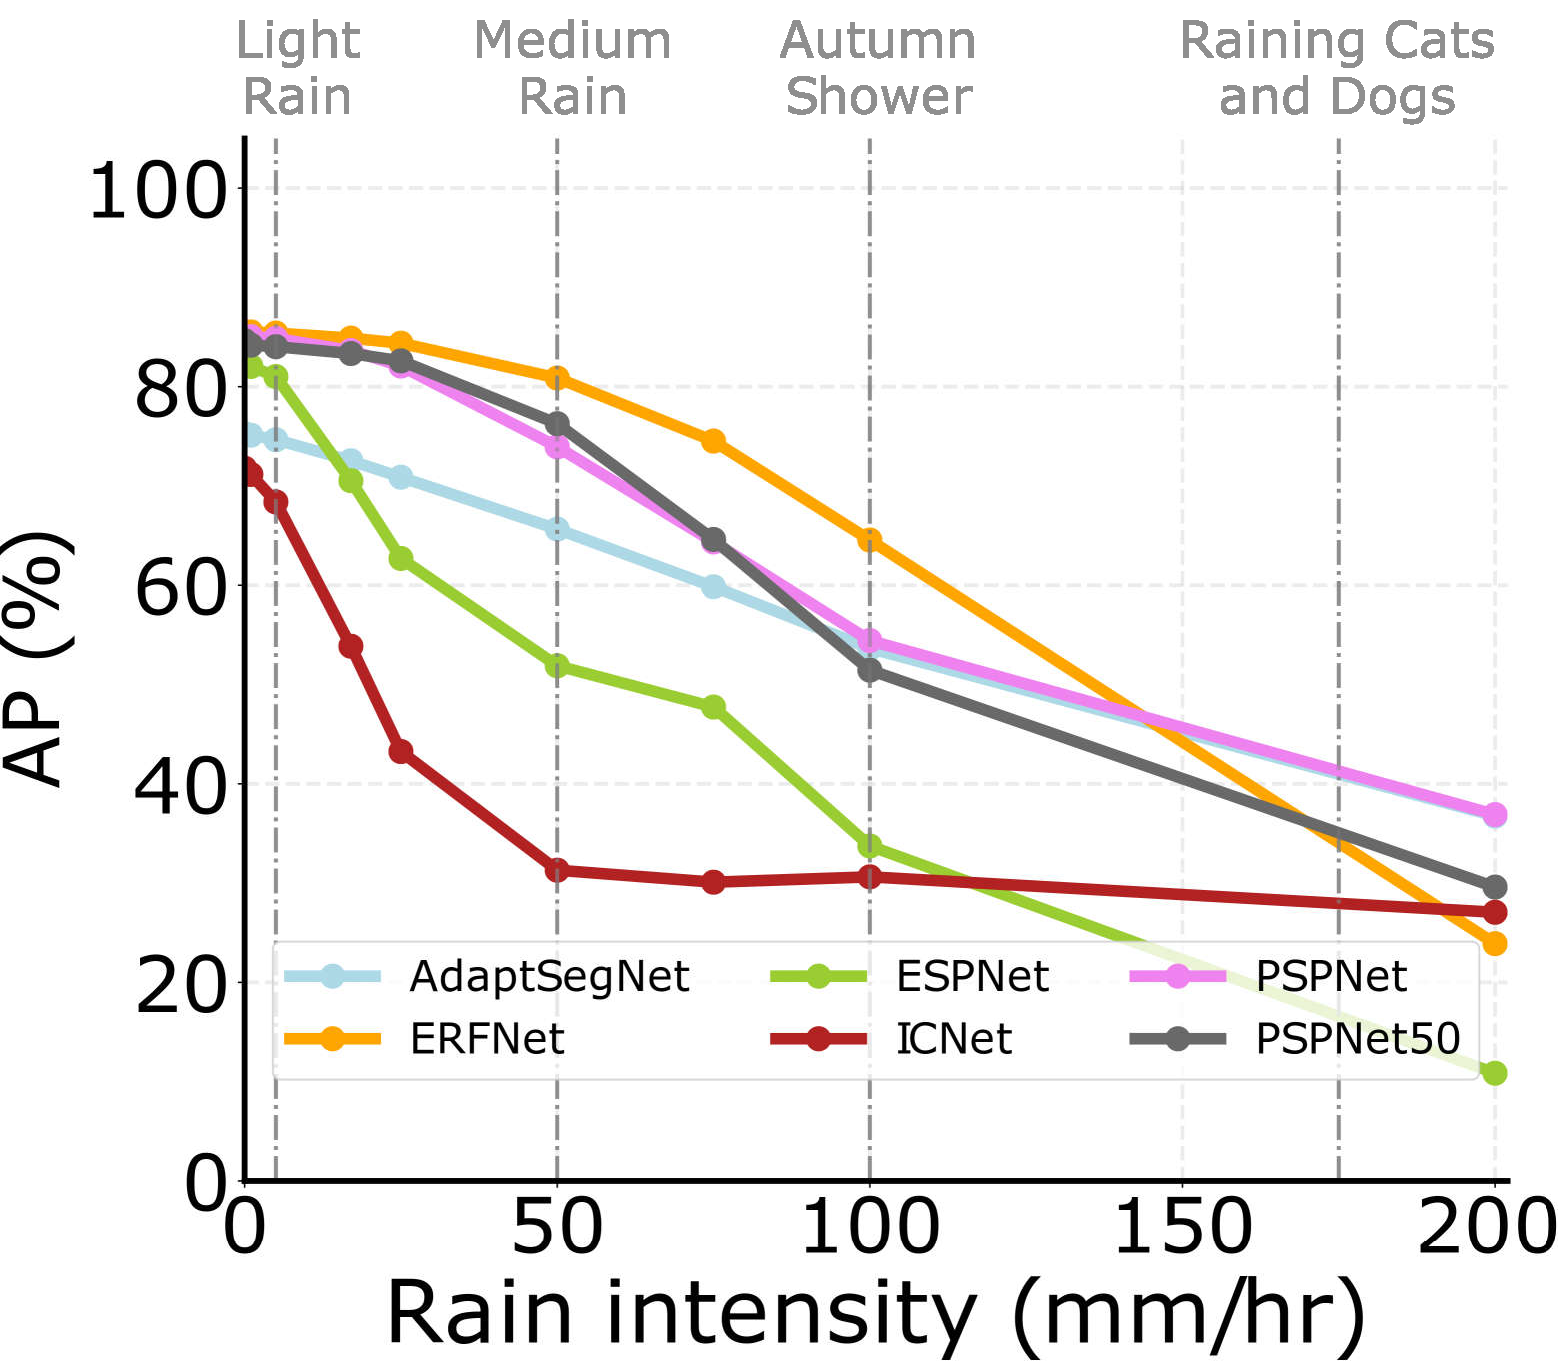
\includegraphics[width=0.485\linewidth]{figures/plots/sem_segm_perf_rain.pdf}\label{fig:algo_sem_seg_perf}}
 \hfill%
 \subfloat[Depth estimation]{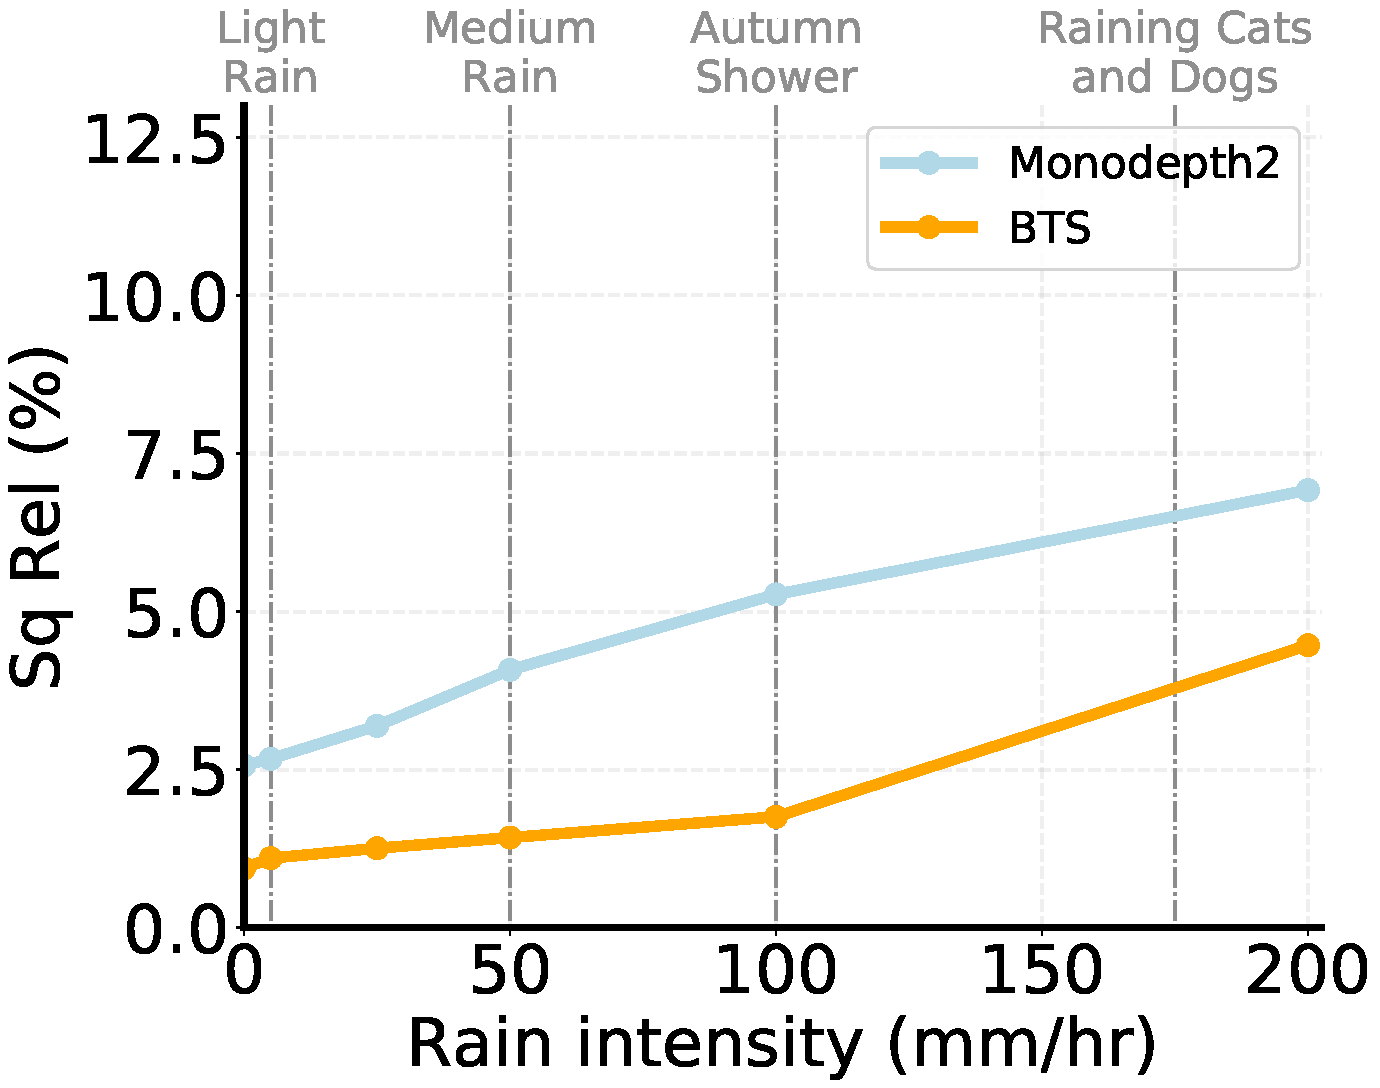
\includegraphics[width=0.485\linewidth]{figures/plots/depth_estim_performances.pdf}\label{fig:algo_depth_estim_perf}}
 \caption{\textbf{Performance using our PBR rain augmentation}. \protect\subref{fig:algo_obj_detect_perf} Object detection performance on our weather augmented KITTI dataset, \protect\subref{fig:algo_sem_seg_perf} pixel-semantic segmentation performance on our weather augmented Cityscapes dataset, and \protect\subref{fig:algo_depth_estim_perf} depth estimation performance on our weather augmented nuScenes dataset, all of them as a function of rainfall rate. The object detection plot shows the Coco mAP@[.1:.1:.9] (\%) across cars and pedestrians, the semantic segmentation plot shows the AP (\%), and the depth estimation shows the squared relative error (\%). As opposed to object detection which exhibits some robustness, the segmentation and depth estimation tasks are strongly affected by the rain.}
 \label{fig:obj_sem_depth_rain_perf}
\end{figure}

\subsection{Evaluating PBR rain augmentation}

\newcommand\weatherAugmented[4]{
 \adjincludegraphics[width=0.222\linewidth, trim={{0.28346456692\width} 3px {0.12047244094\width} 2px}, clip]{figures/results/qualitative_rain/#2/clear/#1.#3} \hspace{0.085em} &
 \adjincludegraphics[width=0.222\linewidth, trim={{0.28346456692\width} 0 {0.12047244094\width} 0}, clip]{figures/results/qualitative_rain/#2/pbr/50mm/#1.#4} &  
 \adjincludegraphics[width=0.222\linewidth, trim={{0.28346456692\width} 0 {0.12047244094\width} 0}, clip]{figures/results/qualitative_rain/#2/pbr/100mm/#1.#4} & 
 \adjincludegraphics[width=0.222\linewidth, trim={{0.28346456692\width} 0 {0.12047244094\width} 0}, clip]{figures/results/qualitative_rain/#2/pbr/200mm/#1.#4}}

\newcommand\weatherHybridAugmented[4]{
 \adjincludegraphics[width=0.191\linewidth]{figures/results/qualitative_rain/#2/clear_small/#1.#3} \hspace{0.085em} &
 \adjincludegraphics[width=0.191\linewidth]{figures/results/qualitative_rain/#2/gan/#1.#4} &
 \adjincludegraphics[width=0.191\linewidth]{figures/results/qualitative_rain/#2/hybrid/50mm/#1.#4} & 
 \adjincludegraphics[width=0.191\linewidth]{figures/results/qualitative_rain/#2/hybrid/100mm/#1.#4} & 
 \adjincludegraphics[width=0.191\linewidth]{figures/results/qualitative_rain/#2/hybrid/200mm/#1.#4}}


\begin{figure*}
 \newcommand\weatheraugvizObjDetT[3]{
  \adjincludegraphics[width=0.222\linewidth, trim={{0.28346456692\width} 0 {0.12047244094\width} 0}, clip]{figures/results/obj_detection/#2/#1#3_clear_tb.jpg} \hspace{0.085em} & 
  \adjincludegraphics[width=0.222\linewidth, trim={{0.28346456692\width} 0 {0.12047244094\width} 0}, clip]{figures/results/obj_detection/#2/#1#3_50mm_tb.jpg} & 
  \adjincludegraphics[width=0.222\linewidth, trim={{0.28346456692\width} 0 {0.12047244094\width} 0}, clip]{figures/results/obj_detection/#2/#1#3_100mm_tb.jpg} &
  \adjincludegraphics[width=0.222\linewidth, trim={{0.28346456692\width} 0 {0.12047244094\width} 0}, clip]{figures/results/obj_detection/#2/#1#3_200mm_tb.jpg}}
 \newcommand\weatheraugvizObjDet[2]{\weatheraugvizObjDetT{#1}{#2}{_#2}}
 
 \centering
 \scriptsize
 \setlength{\tabcolsep}{0.001\linewidth}
 \renewcommand{\arraystretch}{0.5}
 \begin{tabular}{ccccc}
  & \textbf{\footnotesize{Original}} & \multicolumn{3}{c}{\textbf{\footnotesize{Rain augmented (PBR)}}} \\
  \cmidrule[1pt](l{2pt}r{4pt}){2-2}\cmidrule[1pt](l{2pt}r{2pt}){3-5}
  \multirow{1}{*}[1.15cm]{\rotatebox{90}{Input}} & 
	 \adjincludegraphics[width=0.222\linewidth, trim={{0.28346456692\width} 3px {0.12047244094\width} 2px}, clip]{figures/results/qualitative_rain/kitti/clear/000095_tb.jpg} \hspace{0.085em} &
   \adjincludegraphics[width=0.222\linewidth, trim={{0.28346456692\width} 0 {0.12047244094\width} 0}, clip]{figures/results/qualitative_rain/kitti/pbr/50mm/000095_tb.jpg} &  
   \adjincludegraphics[width=0.222\linewidth, trim={{0.28346456692\width} 0 {0.12047244094\width} 0}, clip]{figures/results/qualitative_rain/kitti/pbr/100mm/000095_tb.jpg} & 
   \adjincludegraphics[width=0.222\linewidth, trim={{0.28346456692\width} 0 {0.12047244094\width} 0}, clip]{figures/results/qualitative_rain/kitti/pbr/200mm/000095_tb.jpg} \\

  \multirow{1}{*}[1.45cm]{\rotatebox{90}{FasterRCNN} \rotatebox{90}{~~~~~~\cite{ren2015faster}}} & 
	  \adjincludegraphics[width=0.222\linewidth, trim={{0.28346456692\width} 0 {0.12047244094\width} 0}, clip]{figures/results/obj_detection/FasterRCNN/000095_FasterRCNN_clear_tb.jpg} \hspace{0.085em} & 
    \adjincludegraphics[width=0.222\linewidth, trim={{0.28346456692\width} 0 {0.12047244094\width} 0}, clip]{figures/results/obj_detection/FasterRCNN/000095_FasterRCNN_50mm_tb.jpg} & 
    \adjincludegraphics[width=0.222\linewidth, trim={{0.28346456692\width} 0 {0.12047244094\width} 0}, clip]{figures/results/obj_detection/FasterRCNN/000095_FasterRCNN_100mm_tb.jpg} &
    \adjincludegraphics[width=0.222\linewidth, trim={{0.28346456692\width} 0 {0.12047244094\width} 0}, clip]{figures/results/obj_detection/FasterRCNN/000095_FasterRCNN_200mm_tb.jpg} \\
	
  \multirow{1}{*}[1.15cm]{\rotatebox{90}{R-FCN} \rotatebox{90}{~~\cite{dai2016r}}} & 
	\adjincludegraphics[width=0.222\linewidth, trim={{0.28346456692\width} 0 {0.12047244094\width} 0}, clip]{figures/results/obj_detection/RFCN/000095_RFCN_clear_tb.jpg} \hspace{0.085em} & 
  \adjincludegraphics[width=0.222\linewidth, trim={{0.28346456692\width} 0 {0.12047244094\width} 0}, clip]{figures/results/obj_detection/RFCN/000095_RFCN_50mm_tb.jpg} & 
  \adjincludegraphics[width=0.222\linewidth, trim={{0.28346456692\width} 0 {0.12047244094\width} 0}, clip]{figures/results/obj_detection/RFCN/000095_RFCN_100mm_tb.jpg} &
  \adjincludegraphics[width=0.222\linewidth, trim={{0.28346456692\width} 0 {0.12047244094\width} 0}, clip]{figures/results/obj_detection/RFCN/000095_RFCN_200mm_tb.jpg} \\
	
  \multirow{1}{*}[1.35cm]{\rotatebox{90}{MX-RCNN} \rotatebox{90}{~~~~~~\cite{yang2016exploit}}} & 
	\adjincludegraphics[width=0.222\linewidth, trim={{0.28346456692\width} 0 {0.12047244094\width} 0}, clip]{figures/results/obj_detection/MxRCNN/000095_MxRCNN_clear_tb.jpg} \hspace{0.085em} & 
  \adjincludegraphics[width=0.222\linewidth, trim={{0.28346456692\width} 0 {0.12047244094\width} 0}, clip]{figures/results/obj_detection/MxRCNN/000095_MxRCNN_50mm_tb.jpg} & 
  \adjincludegraphics[width=0.222\linewidth, trim={{0.28346456692\width} 0 {0.12047244094\width} 0}, clip]{figures/results/obj_detection/MxRCNN/000095_MxRCNN_100mm_tb.jpg} &
  \adjincludegraphics[width=0.222\linewidth, trim={{0.28346456692\width} 0 {0.12047244094\width} 0}, clip]{figures/results/obj_detection/MxRCNN/000095_MxRCNN_200mm_tb.jpg} \\
	
  \multirow{1}{*}[1.25cm]{\rotatebox{90}{YOLOv2} \rotatebox{90}{~~~~\cite{redmon2017yolo9000}}} & 
	\adjincludegraphics[width=0.222\linewidth, trim={{0.28346456692\width} 0 {0.12047244094\width} 0}, clip]{figures/results/obj_detection/YoloV2/000095_YoloV2_clear_tb.jpg} \hspace{0.085em} & 
  \adjincludegraphics[width=0.222\linewidth, trim={{0.28346456692\width} 0 {0.12047244094\width} 0}, clip]{figures/results/obj_detection/YoloV2/000095_YoloV2_50mm_tb.jpg} & 
  \adjincludegraphics[width=0.222\linewidth, trim={{0.28346456692\width} 0 {0.12047244094\width} 0}, clip]{figures/results/obj_detection/YoloV2/000095_YoloV2_100mm_tb.jpg} &
  \adjincludegraphics[width=0.222\linewidth, trim={{0.28346456692\width} 0 {0.12047244094\width} 0}, clip]{figures/results/obj_detection/YoloV2/000095_YoloV2_200mm_tb.jpg} \\
	
  & Clear weather & Moderate rain & Heavy rain     & Shower rain \\
  &    & (50~mm/hr)  & (100~mm/hr)   & (200~mm/hr) \\
 \end{tabular}
 \caption{\textbf{Object detection on PBR rain augmentation of KITTI.} From left to right, the original image (clear) and three PBR augmentations with varying rainfall rates. Images are cropped for visualization.}
 \label{fig:eval_qualitative_objdet}
\end{figure*}

\renewcommand\weatherAugmented[4]{
 \adjincludegraphics[width=0.222\linewidth]{figures/results/qualitative_rain/#2/clear/#1.#3} \hspace{0.085em} &
 \adjincludegraphics[width=0.222\linewidth]{figures/results/qualitative_rain/#2/pbr/50mm/#1.#4} & 
 \adjincludegraphics[width=0.222\linewidth]{figures/results/qualitative_rain/#2/pbr/100mm/#1.#4} & 
 \adjincludegraphics[width=0.222\linewidth]{figures/results/qualitative_rain/#2/pbr/200mm/#1.#4}}

\begin{figure*}
 \newcommand\weatheraugvizSegT[4]{
  \includegraphics[width=0.222\linewidth]{figures/results/semantic_seg/#2/#1#3_clear_tb.#4} \hspace{0.085em} & 
  \includegraphics[width=0.222\linewidth]{figures/results/semantic_seg/#2/#1#3_50mm_tb.#4} & 
  \includegraphics[width=0.222\linewidth]{figures/results/semantic_seg/#2/#1#3_100mm_tb.#4} & 
  \includegraphics[width=0.222\linewidth]{figures/results/semantic_seg/#2/#1#3_200mm_tb.#4}}
 \newcommand\weatheraugvizSeg[2]{\weatheraugvizSegT{#1}{#2}{_#2}{png}}
 
 \centering
 \scriptsize
 \setlength{\tabcolsep}{0.001\linewidth}
 \renewcommand{\arraystretch}{0.5}
 \begin{tabular}{ccccc}
  & \textbf{\footnotesize{Original}}&\multicolumn{3}{c}{\textbf{\footnotesize{Rain augmented (PBR)}}} \\
  \cmidrule[1pt](l{2pt}r{4pt}){2-2}\cmidrule[1pt](l{2pt}r{2pt}){3-5}
  \multirow{1}{*}[1.1cm]{\rotatebox{90}{Input}} & 
	\adjincludegraphics[width=0.222\linewidth]{figures/results/qualitative_rain/cityscapes/clear/bochum_000000_016260_leftImg8bit_tb.jpg} \hspace{0.085em} &
 \adjincludegraphics[width=0.222\linewidth]{figures/results/qualitative_rain/cityscapes/pbr/50mm/bochum_000000_016260_leftImg8bit_tb.jpg} & 
 \adjincludegraphics[width=0.222\linewidth]{figures/results/qualitative_rain/cityscapes/pbr/100mm/bochum_000000_016260_leftImg8bit_tb.jpg} & 
 \adjincludegraphics[width=0.222\linewidth]{figures/results/qualitative_rain/cityscapes/pbr/200mm/bochum_000000_016260_leftImg8bit_tb.jpg} \\
	
  \multirow{1}{*}[1.25cm]{\rotatebox{90}{ERFNet} \rotatebox{90}{~~~\cite{romera2018erfnet}}} &
	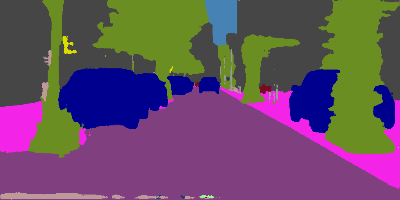
\includegraphics[width=0.222\linewidth]{figures/results/semantic_seg/ERFNet/bochum_000000_016260_leftImg8bit_ERFNet_clear_tb.png} \hspace{0.085em} & 
  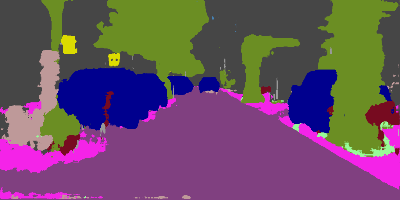
\includegraphics[width=0.222\linewidth]{figures/results/semantic_seg/ERFNet/bochum_000000_016260_leftImg8bit_ERFNet_50mm_tb.png} & 
  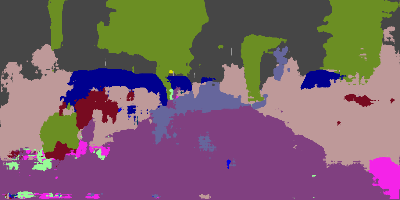
\includegraphics[width=0.222\linewidth]{figures/results/semantic_seg/ERFNet/bochum_000000_016260_leftImg8bit_ERFNet_100mm_tb.png} & 
  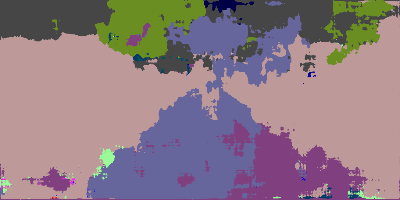
\includegraphics[width=0.222\linewidth]{figures/results/semantic_seg/ERFNet/bochum_000000_016260_leftImg8bit_ERFNet_200mm_tb.png} \\
	
  \multirow{1}{*}[1.25cm]{\rotatebox{90}{ESPNet} \rotatebox{90}{~~~\cite{mehta2018espnet}}} & 
	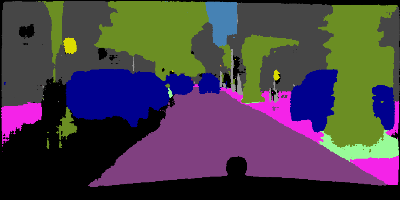
\includegraphics[width=0.222\linewidth]{figures/results/semantic_seg/ESPNet/bochum_000000_016260_leftImg8bit_ESPNet_clear_tb.png} \hspace{0.085em} & 
  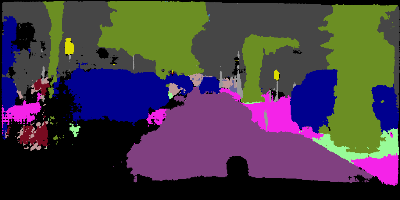
\includegraphics[width=0.222\linewidth]{figures/results/semantic_seg/ESPNet/bochum_000000_016260_leftImg8bit_ESPNet_50mm_tb.png} & 
  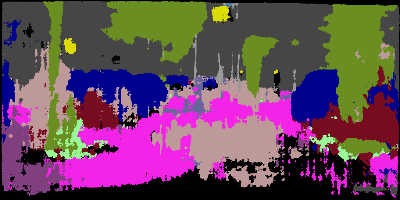
\includegraphics[width=0.222\linewidth]{figures/results/semantic_seg/ESPNet/bochum_000000_016260_leftImg8bit_ESPNet_100mm_tb.png} & 
  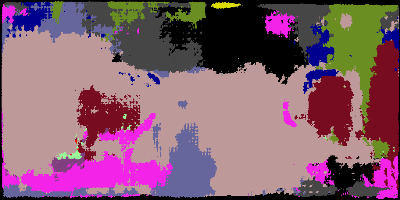
\includegraphics[width=0.222\linewidth]{figures/results/semantic_seg/ESPNet/bochum_000000_016260_leftImg8bit_ESPNet_200mm_tb.png} \\
	
  \multirow{1}{*}[1.25cm]{\rotatebox{90}{ICNet} \rotatebox{90}{~\cite{zhao2018icnet}}} & 
	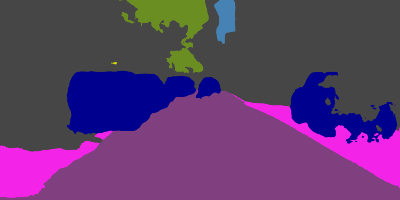
\includegraphics[width=0.222\linewidth]{figures/results/semantic_seg/ICNet/bochum_000000_016260_leftImg8bit_ICNet_clear_tb.png} \hspace{0.085em} & 
  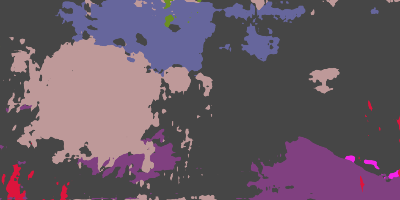
\includegraphics[width=0.222\linewidth]{figures/results/semantic_seg/ICNet/bochum_000000_016260_leftImg8bit_ICNet_50mm_tb.png} & 
  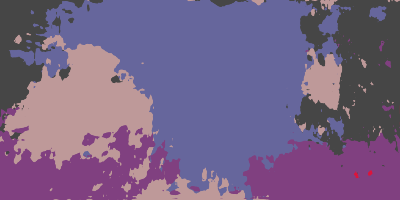
\includegraphics[width=0.222\linewidth]{figures/results/semantic_seg/ICNet/bochum_000000_016260_leftImg8bit_ICNet_100mm_tb.png} & 
  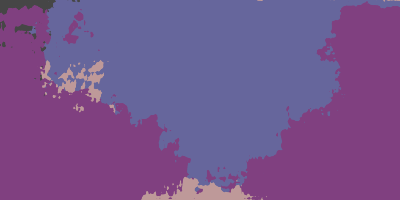
\includegraphics[width=0.222\linewidth]{figures/results/semantic_seg/ICNet/bochum_000000_016260_leftImg8bit_ICNet_200mm_tb.png} \\
	
  \multirow{1}{*}[1.25cm]{\rotatebox{90}{PSPNet} \rotatebox{90}{~~~\cite{zhao2017pspnet}}} & 
	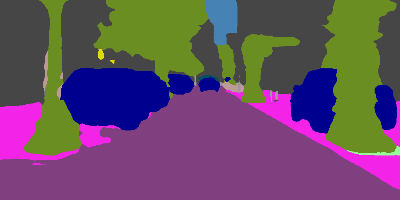
\includegraphics[width=0.222\linewidth]{figures/results/semantic_seg/PSPNet/bochum_000000_016260_leftImg8bit_PSPNet_clear_tb.png} \hspace{0.085em} & 
  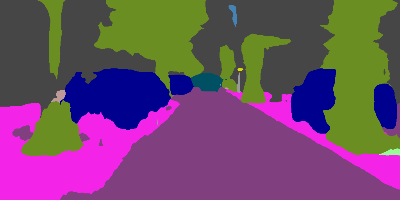
\includegraphics[width=0.222\linewidth]{figures/results/semantic_seg/PSPNet/bochum_000000_016260_leftImg8bit_PSPNet_50mm_tb.png} & 
  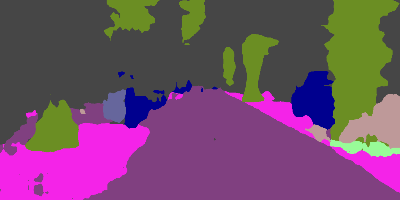
\includegraphics[width=0.222\linewidth]{figures/results/semantic_seg/PSPNet/bochum_000000_016260_leftImg8bit_PSPNet_100mm_tb.png} & 
  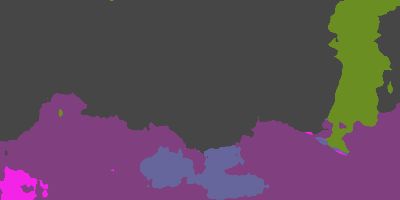
\includegraphics[width=0.222\linewidth]{figures/results/semantic_seg/PSPNet/bochum_000000_016260_leftImg8bit_PSPNet_200mm_tb.png} \\
	
  &Clear weather  & Moderate rain  & Heavy rain  & Shower rain \\
  &    & (50~mm/hr)        & (100~mm/hr)  & (200~mm/hr) \\
 \end{tabular}
 \caption{\textbf{Qualitative evaluation of semantic segmentation on our PBR rain augmentation of Cityscapes.} From left to right, the original image (clear) and three PBR augmentations with varying rainfall rates.}
 \label{fig:eval_qualitative_seg}
\end{figure*}

\begin{figure*}
 \newcommand\weatheraugvizDepthEstimT[3]{
  \includegraphics[width=0.222\linewidth]{figures/results/depth_estim/#2/clear/#1.#3} \hspace{0.085em} & 
  \includegraphics[width=0.222\linewidth]{figures/results/depth_estim/#2/50mm/#1.#3} & 
  \includegraphics[width=0.222\linewidth]{figures/results/depth_estim/#2/100mm/#1.#3} & 
  \includegraphics[width=0.222\linewidth]{figures/results/depth_estim/#2/200mm/#1.#3}}
 
 \centering
 \scriptsize
 \setlength{\tabcolsep}{0.001\linewidth}
 \renewcommand{\arraystretch}{0.5}
 \begin{tabular}{ccccc}
  & \textbf{\footnotesize{Original}}&\multicolumn{3}{c}{\textbf{\footnotesize{Rain augmented (PBR)}}} \\
  \cmidrule[1pt](l{2pt}r{4pt}){2-2}\cmidrule[1pt](l{2pt}r{2pt}){3-5}
  \multirow{1}{*}[1.25cm]{\rotatebox{90}{Input}} & 
	\adjincludegraphics[width=0.222\linewidth]{figures/results/qualitative_rain/nuscenes/clear/008.jpg} \hspace{0.085em} &
  \adjincludegraphics[width=0.222\linewidth]{figures/results/qualitative_rain/nuscenes/pbr/50mm/008.png} & 
  \adjincludegraphics[width=0.222\linewidth]{figures/results/qualitative_rain/nuscenes/pbr/100mm/008.png} & 
  \adjincludegraphics[width=0.222\linewidth]{figures/results/qualitative_rain/nuscenes/pbr/200mm/008.png} \\
	
  \multirow{1}{*}[1.7cm]{\rotatebox{90}{Monodepth2} \rotatebox{90}{~~~~~~~\cite{godard2019digging}}} &
	
\includegraphics[width=0.222\linewidth]{figures/results/depth_estim/monodepth2/clear/008.png} \hspace{0.085em} & 
  
\includegraphics[width=0.222\linewidth]{figures/results/depth_estim/monodepth2/50mm/008.png} & 
  
\includegraphics[width=0.222\linewidth]{figures/results/depth_estim/monodepth2/100mm/008.png} & 
  
\includegraphics[width=0.222\linewidth]{figures/results/depth_estim/monodepth2/200mm/008.png} \\
	
  \multirow{1}{*}[1.2cm]{\rotatebox{90}{BTS} \rotatebox{90}{\cite{lee2020big}}} &
	
\includegraphics[width=0.222\linewidth]{figures/results/depth_estim/bts/clear/008.png} \hspace{0.085em} & 
  
\includegraphics[width=0.222\linewidth]{figures/results/depth_estim/bts/50mm/008.png} & 
  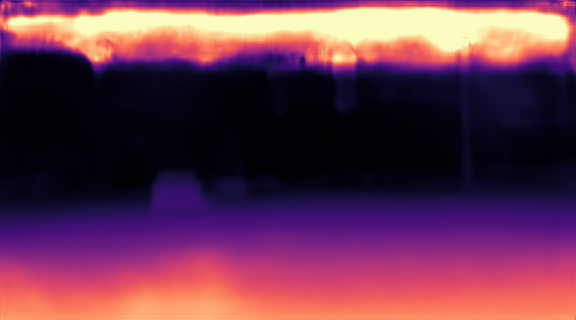
\includegraphics[width=0.222\linewidth]{figures/results/depth_estim/bts/100mm/008.png} & 
  
\includegraphics[width=0.222\linewidth]{figures/results/depth_estim/bts/200mm/008.png} \\
		
  &Clear weather  & Moderate rain  & Heavy rain  & Shower rain \\
  &    & (50~mm/hr)        & (100~mm/hr)  & (200~mm/hr) \\
 \end{tabular}
 \caption{\textbf{Depth estimation on our PBR rain augmentation of nuScenes.} From left to right, the original image (clear) and three PBR augmentations with varying rainfall rates.}
 \label{fig:eval_qualitative_depthestm}
\end{figure*}

We compare the performance on PBR-augmented images for 6~object detection algorithms on KITTI~\cite{Geiger2012CVPR}~(7481 images), 6~segmentation algorithms on Cityscapes~\cite{Cordts2016Cityscapes}~(2995 images) and 2 depth estimation algorithm on nuScenes-augment~(4449 images). 
For all of the algorithms, the clear version always serves as a baseline to which we compare the performance on synthetic rain translations.

\paragraph{Object detection.}
We evaluate the 6 PBR augmented weathers on KITTI for 6~car/pedestrian pre-trained detection algorithms (with $\text{IoU}\geq.7$): DSOD~\cite{Shen2017DSOD}, Faster R-CNN~\cite{ren2015faster}, R-FCN~\cite{dai2016r}, SSD~\cite{liu2016ssd}, MX-RCNN~\cite{yang2016exploit}, and YOLOv2~\cite{redmon2017yolo9000}. Quantitative results for the Coco mAP@[.1:.1:.9] metric across classes are shown in fig.~\ref{fig:algo_obj_detect_perf}. Relative to their clear-weather performance the 200~mm/hr rain is always at least 12\% worse and even drops to 25-30\% for R-FCN, SSD, and MX-RCNN, whereas Faster R-CNN and DSOD are the most robust to changes in fog and rain. 

Representative qualitative results on PBR images are shown in fig.~\ref{fig:eval_qualitative_objdet} for 4 out of 6 algorithms to preserve space. All algorithms are strongly affected by the rain; it has a chaotic effect on object detection results because there can be large variance of occlusion level for objects populating the image. Also, as in real-life, far away objects (which are generally small objects) are more likely to disappear behind fog-like rain. 

\paragraph{Semantic segmentation.}
For semantic segmentation, the PBR augmented Cityscapes is evaluated for: AdaptSegNet~\cite{Tsai_adaptseg_2018}, ERFNet~\cite{romera2018erfnet}, ESPNet~\cite{mehta2018espnet}, ICNet~\cite{zhao2018icnet}, PSPNet~\cite{zhao2017pspnet} and PSPNet(50)~\cite{zhao2017pspnet}.
Quantitative results are reported in fig.~\ref{fig:algo_sem_seg_perf}. As opposed to object detection algorithms which demonstrated significant robustness to moderately high rainfall rates, here the algorithms seem to breakdown in similar conditions. Indeed, all techniques see their performance drop by a minimum of 30\% under heavy fog, and almost 60\% under strong rain. Interestingly, some curves cross, which indicates that different algorithms behave differently under rain. ESPNet for example, ranks among the top 3 in clear weather but drops relatively by a staggering 85\% and ranks last in stormy conditions (200mm/hr). Corresponding qualitative results are shown in fig.~\ref{fig:eval_qualitative_seg} for 4 out of 6 algorithms to preserve space. Although the effect of rain may appear minimal visually, it greatly affects the output of all segmentation algorithms evaluated. 

\paragraph{Depth estimation.}
We evaluate the performance of the recent Monodepth2~\cite{godard2019digging} and BTS~\cite{lee2020big} on the nuScenes-augment subset augmented with our PBR method.
We report the standard squared relative error in fig.~\ref{fig:algo_depth_estim_perf} and note that the error seems to increase linearly with rain. In the extreme 200mm/hr rain conditions, we measure an error of 3x that of clear images.
Qualitative results are shown in fig.~\ref{fig:eval_qualitative_depthestm}. It can be observed that performance drops when raindrops block the view or fog-like limits the visibility in the image.

\subsection{Evaluating GAN and GAN+PBR rain augmentations}

Next, we ascertain the effect of the rain augmentation with our GAN and GAN+PBR augmentation strategies. As mentioned above, semantic segmentation algorithms are not evaluated due to the lack of semantic labels for training. The evaluation is performed on the nuScenes-augment subset. 

\paragraph{Object detection.}
YOLOv2~\cite{redmon2017yolo9000} is evaluated, and the resulting mAP as a function of rainfall rates are reported in fig.~\ref{fig:hybrid_obj_detect_perf}. Qualitative results are shown in fig.~\ref{fig:eval_obj_detect_qualitative_hybrid}. We note that GAN augmented images have similar performance than PBR 100mm/hr images and that performance deterioration is stronger and steeper with GAN+PBR images. 

Observe that the particles physical simulation is the same in both PBR and GAN+PBR. Still, it is interesting to notice that the decrease is different with GAN+PBR compared to PBR (i.e. curves are shifted but also exhibit different slopes). This may be the result of the two cumulative domain shifts (i.e. wetness + streaks) leading to a non-linear effect.

\paragraph{Depth estimation.}
We evaluate the performance of the recent Monodepth2~\cite{godard2019digging} on the nuScenes-augment subset augmented with our GAN and GAN+PBR methods. 
As reported in fig.~\ref{fig:hybrid_depth_estim_perf}, for the same rain intensity between PBR and GAN+PBR images, the error is worse by a factor of 80--100\%. The same behavior was observed on other standard depth estimation metrics (absolute square error, RMSE, log RMSE), not reported here. Interestingly, the GAN augmentation affects only slightly the performance on depth estimation which might be because GAN translation keeps occlusion of the image to a minimum.
Qualitative results are shown in fig.~\ref{fig:eval_depth_estim_detect_qualitative_hybrid} for GAN and GAN+PBR. 

\begin{figure}
 \centering
 \subfloat[Object detection~\cite{redmon2017yolo9000}]{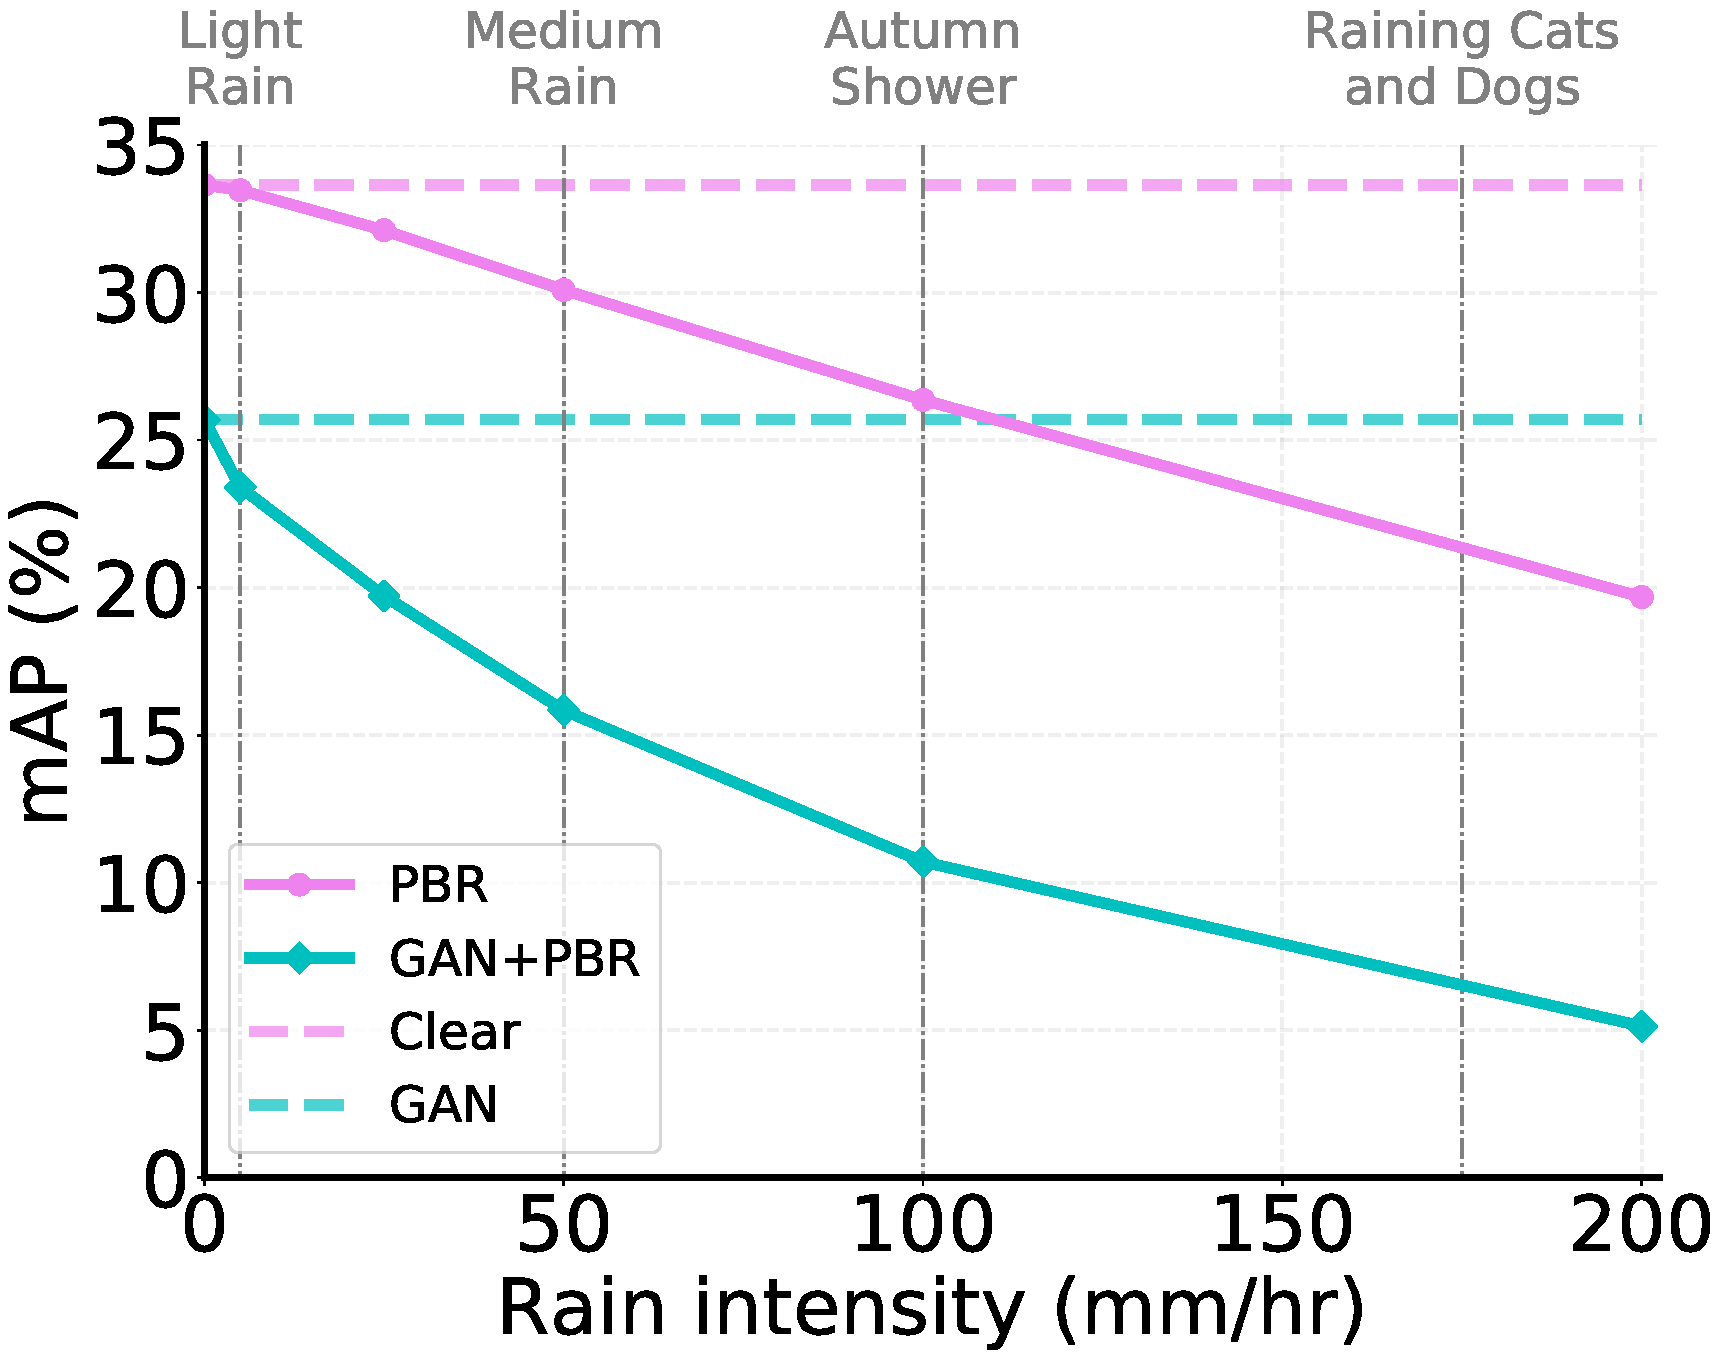
\includegraphics[width=0.485\linewidth]{figures/plots/yolov2_hybrid_performances.pdf} \label{fig:hybrid_obj_detect_perf}}\hfill%
    \subfloat[Depth estimation~\cite{godard2019digging}]{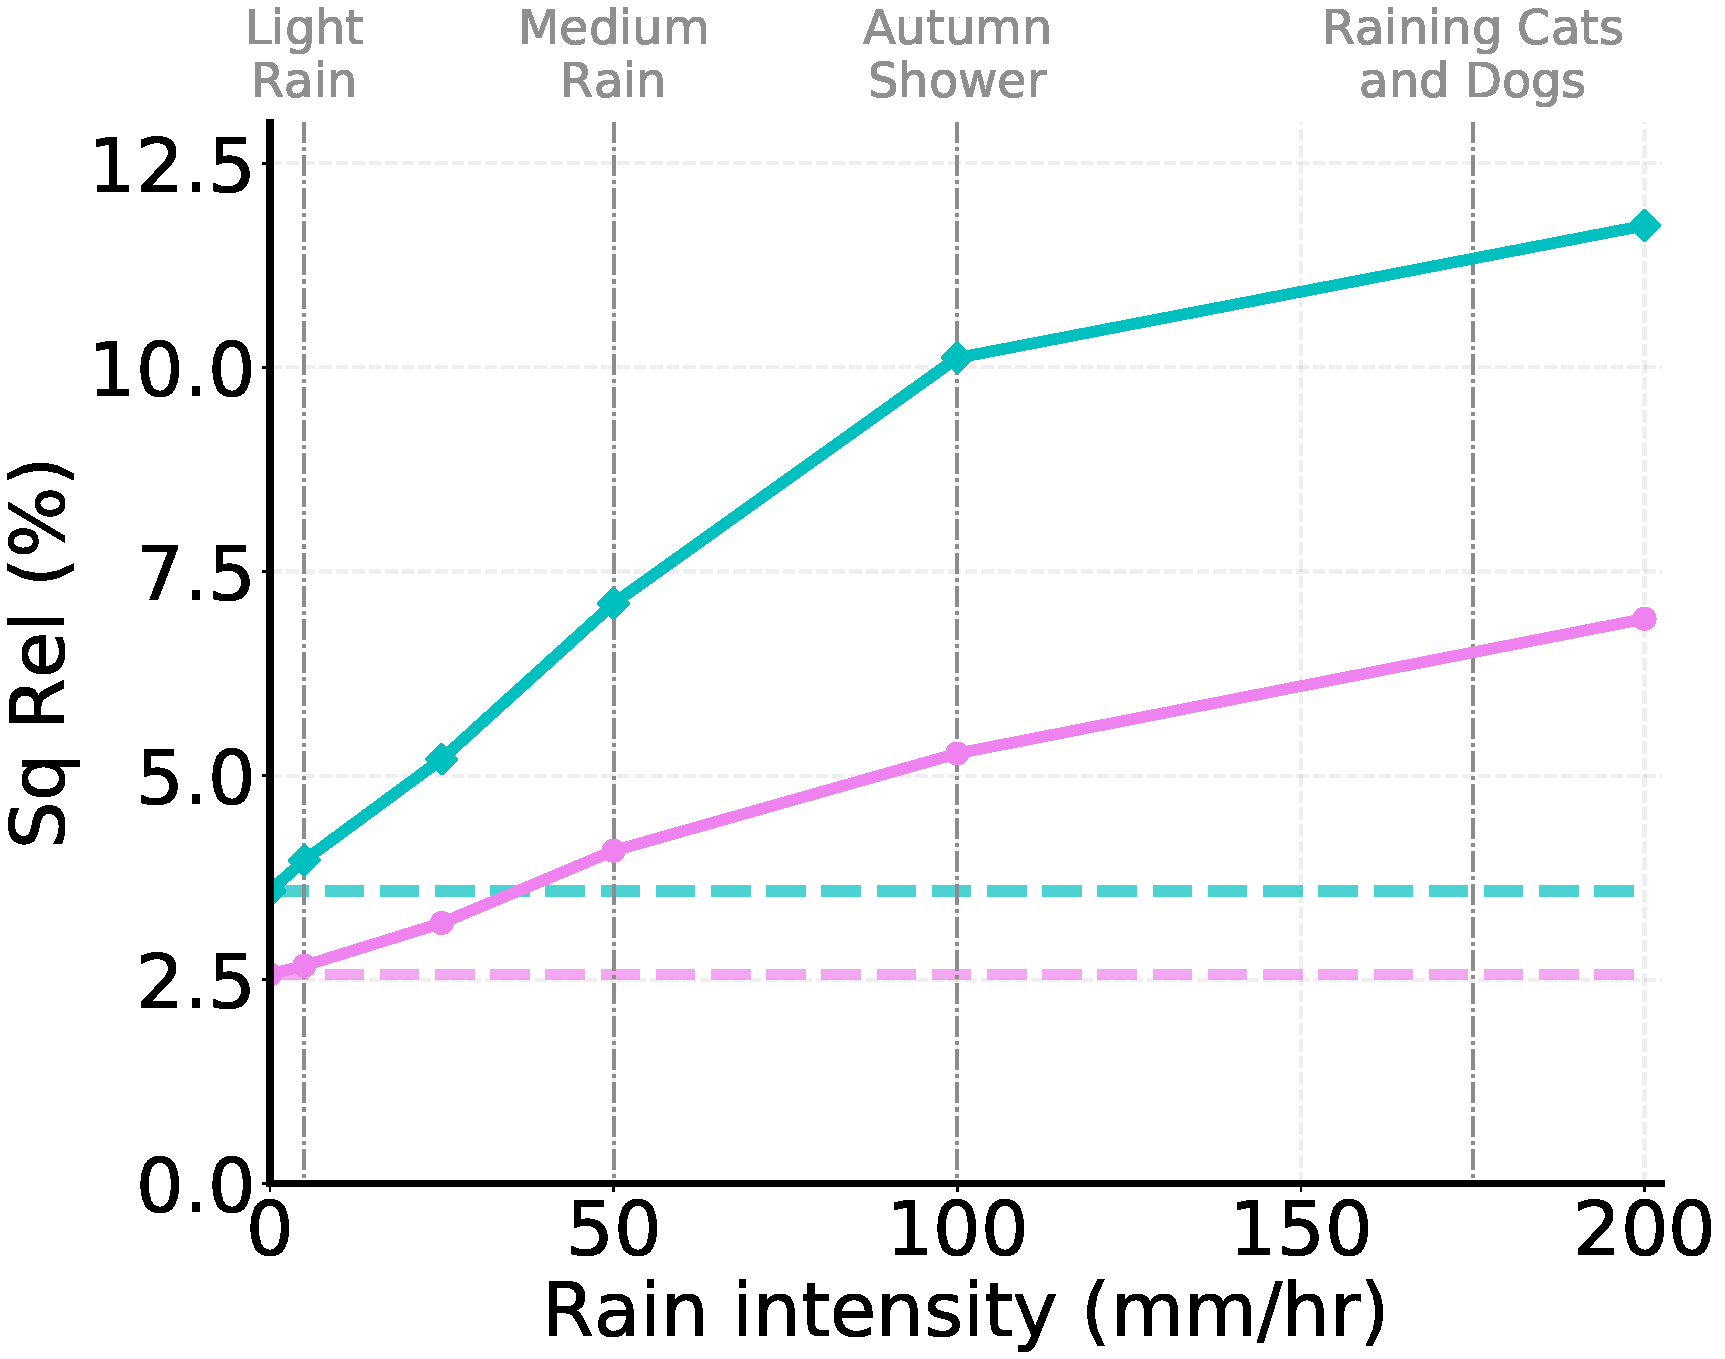
\includegraphics[width=0.485\linewidth]{figures/plots/monodepth2_hybrid_performances.pdf} \label{fig:hybrid_depth_estim_perf}} 
 \caption{\textbf{Performance with varying rain intensities and augmentation techniques.} Opposed to PBR, GAN does not allow to control the rain intensity and is reported as dashed line, as for clear performance. Increasing rain intensity translates as a performance drop for \protect\subref{fig:hybrid_obj_detect_perf} object detection with YOLOv2~\cite{redmon2017yolo9000} and \protect\subref{fig:hybrid_depth_estim_perf} depth estimation with Monodepth2~\cite{godard2019digging}.}
 \label{fig:hybrid_perf}
\end{figure}

\begin{figure*}
 \newcommand\weatheraugvizHybridExp[2]{
 \includegraphics[width=0.191\linewidth]{figures/results/hybrid/#2/clear/#1.png} \hspace{0.085em} &
 \includegraphics[width=0.191\linewidth]{figures/results/hybrid/#2/gan/#1.png} &
 \includegraphics[width=0.191\linewidth]{figures/results/hybrid/#2/50mm/#1.png} & 
 \includegraphics[width=0.191\linewidth]{figures/results/hybrid/#2/100mm/#1.png} & 
 \includegraphics[width=0.191\linewidth]{figures/results/hybrid/#2/200mm/#1.png}}
 
 \centering
 \scriptsize
 \setlength{\tabcolsep}{0.001\linewidth}
 \renewcommand{\arraystretch}{0.5}
 \begin{tabular}{cccccc}
  & \textbf{\footnotesize{Original}}&\multicolumn{4}{c}{\textbf{\footnotesize{Rain augmented (GAN+PBR)}}} \\
  \cmidrule[1pt](l{2pt}r{4pt}){2-2}\cmidrule[1pt](l{2pt}r{2pt}){3-6}
  \multirow{1}{*}[1.15cm]{\rotatebox{90}{Input}} & 
	\adjincludegraphics[width=0.191\linewidth]{figures/results/qualitative_rain/nuscenes/clear_small/004.jpg} \hspace{0.085em} &
  \adjincludegraphics[width=0.191\linewidth]{figures/results/qualitative_rain/nuscenes/gan/004.png} &
  \adjincludegraphics[width=0.191\linewidth]{figures/results/qualitative_rain/nuscenes/hybrid/50mm/004.png} & 
  \adjincludegraphics[width=0.191\linewidth]{figures/results/qualitative_rain/nuscenes/hybrid/100mm/004.png} & 
  \adjincludegraphics[width=0.191\linewidth]{figures/results/qualitative_rain/nuscenes/hybrid/200mm/004.png} \\
	
  \multirow{1}{*}[1.25cm]{\rotatebox{90}{YOLOv2} \rotatebox{90}{~~~\cite{redmon2017yolo9000}}} &
	
\includegraphics[width=0.191\linewidth]{figures/results/hybrid/yolov2/clear/004.png} \hspace{0.085em} &
 
\includegraphics[width=0.191\linewidth]{figures/results/hybrid/yolov2/gan/004.png} &
 
\includegraphics[width=0.191\linewidth]{figures/results/hybrid/yolov2/50mm/004.png} & 
 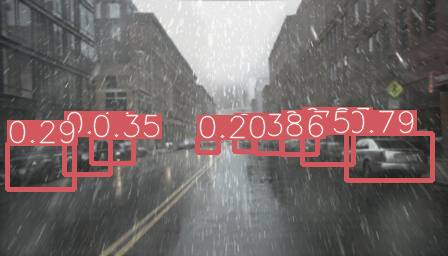
\includegraphics[width=0.191\linewidth]{figures/results/hybrid/yolov2/100mm/004.png} & 
 
\includegraphics[width=0.191\linewidth]{figures/results/hybrid/yolov2/200mm/004.png} \\
	
  \vspace{0.45em} \\
  \multirow{1}{*}[1.15cm]{\rotatebox{90}{Input}} & 
	\adjincludegraphics[width=0.191\linewidth]{figures/results/qualitative_rain/nuscenes/clear_small/002.jpg} \hspace{0.085em} &
  \adjincludegraphics[width=0.191\linewidth]{figures/results/qualitative_rain/nuscenes/gan/002.png} &
  \adjincludegraphics[width=0.191\linewidth]{figures/results/qualitative_rain/nuscenes/hybrid/50mm/002.png} & 
  \adjincludegraphics[width=0.191\linewidth]{figures/results/qualitative_rain/nuscenes/hybrid/100mm/002.png} & 
  \adjincludegraphics[width=0.191\linewidth]{figures/results/qualitative_rain/nuscenes/hybrid/200mm/002.png} \\
	

  \multirow{1}{*}[1.25cm]{\rotatebox{90}{YOLOv2} \rotatebox{90}{~~~\cite{redmon2017yolo9000}}} &
	
\includegraphics[width=0.191\linewidth]{figures/results/hybrid/yolov2/clear/002.png} \hspace{0.085em} &
  
\includegraphics[width=0.191\linewidth]{figures/results/hybrid/yolov2/gan/002.png} &
  
\includegraphics[width=0.191\linewidth]{figures/results/hybrid/yolov2/50mm/002.png} & 
  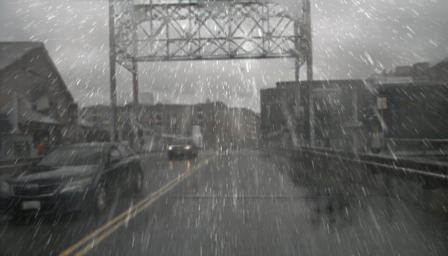
\includegraphics[width=0.191\linewidth]{figures/results/hybrid/yolov2/100mm/002.png} & 
  
\includegraphics[width=0.191\linewidth]{figures/results/hybrid/yolov2/200mm/002.png} \\

  & Clear weather  & GAN only & Moderate rain  & Heavy rain  & Shower rain \\
  &      &     & (50~mm/hr)     & (100~mm/hr)  & (200~mm/hr) \\
 \end{tabular}
 \caption{\textbf{Object detection on our GAN+PBR augmented nuScenes.} From left to right, the original image (clear), the GAN augmented image and three GAN+PBR images.}
 \label{fig:eval_obj_detect_qualitative_hybrid}
\end{figure*}

\begin{figure*}
 \newcommand\weatheraugvizHybridExp[2]{
 \includegraphics[width=0.191\linewidth]{figures/results/hybrid/#2/clear/#1.png} \hspace{0.085em} &
 \includegraphics[width=0.191\linewidth]{figures/results/hybrid/#2/gan/#1.png} &
 \includegraphics[width=0.191\linewidth]{figures/results/hybrid/#2/50mm/#1.png} & 
 \includegraphics[width=0.191\linewidth]{figures/results/hybrid/#2/100mm/#1.png} & 
 \includegraphics[width=0.191\linewidth]{figures/results/hybrid/#2/200mm/#1.png}}
 
 \centering
 \scriptsize
 \setlength{\tabcolsep}{0.001\linewidth}
 \renewcommand{\arraystretch}{0.5}
 \begin{tabular}{cccccc}
  & \textbf{\footnotesize{Original}}&\multicolumn{4}{c}{\textbf{\footnotesize{Rain augmented (GAN+PBR)}}} \\
  \cmidrule[1pt](l{2pt}r{4pt}){2-2}\cmidrule[1pt](l{2pt}r{2pt}){3-6}
  \multirow{1}{*}[1.15cm]{\rotatebox{90}{Input}} & 
	\adjincludegraphics[width=0.191\linewidth]{figures/results/qualitative_rain/nuscenes/clear_small/012.jpg} \hspace{0.085em} &
  \adjincludegraphics[width=0.191\linewidth]{figures/results/qualitative_rain/nuscenes/gan/012.png} &
  \adjincludegraphics[width=0.191\linewidth]{figures/results/qualitative_rain/nuscenes/hybrid/50mm/012.png} & 
  \adjincludegraphics[width=0.191\linewidth]{figures/results/qualitative_rain/nuscenes/hybrid/100mm/012.png} & 
  \adjincludegraphics[width=0.191\linewidth]{figures/results/qualitative_rain/nuscenes/hybrid/200mm/012.png} \\ 
	
  \multirow{1}{*}[1.50cm]{\rotatebox{90}{Monodepth2} \rotatebox{90}{~~~~~\cite{godard2019digging}}} &
	
\includegraphics[width=0.191\linewidth]{figures/results/hybrid/monodepth2/clear/012.png} \hspace{0.085em} &
  
\includegraphics[width=0.191\linewidth]{figures/results/hybrid/monodepth2/gan/012.png} &
  
\includegraphics[width=0.191\linewidth]{figures/results/hybrid/monodepth2/50mm/012.png} & 
  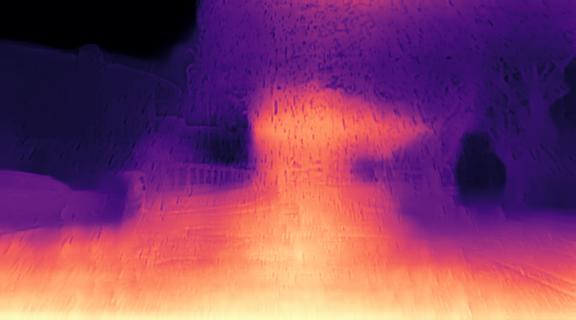
\includegraphics[width=0.191\linewidth]{figures/results/hybrid/monodepth2/100mm/012.png} & 
  
\includegraphics[width=0.191\linewidth]{figures/results/hybrid/monodepth2/200mm/012.png} \\
	
  \vspace{0.45em} \\
  \multirow{1}{*}[1.15cm]{\rotatebox{90}{Input}} & 
	\adjincludegraphics[width=0.191\linewidth]{figures/results/qualitative_rain/nuscenes/clear_small/011.jpg} \hspace{0.085em} &
  \adjincludegraphics[width=0.191\linewidth]{figures/results/qualitative_rain/nuscenes/gan/011.png} &
  \adjincludegraphics[width=0.191\linewidth]{figures/results/qualitative_rain/nuscenes/hybrid/50mm/011.png} & 
  \adjincludegraphics[width=0.191\linewidth]{figures/results/qualitative_rain/nuscenes/hybrid/100mm/011.png} & 
  \adjincludegraphics[width=0.191\linewidth]{figures/results/qualitative_rain/nuscenes/hybrid/200mm/011.png} \\
	
  \multirow{1}{*}[1.50cm]{\rotatebox{90}{Monodepth2} \rotatebox{90}{~~~~~\cite{godard2019digging}}} &
	
\includegraphics[width=0.191\linewidth]{figures/results/hybrid/monodepth2/clear/011.png} \hspace{0.085em} &
  
\includegraphics[width=0.191\linewidth]{figures/results/hybrid/monodepth2/gan/011.png} &
  
\includegraphics[width=0.191\linewidth]{figures/results/hybrid/monodepth2/50mm/011.png} & 
  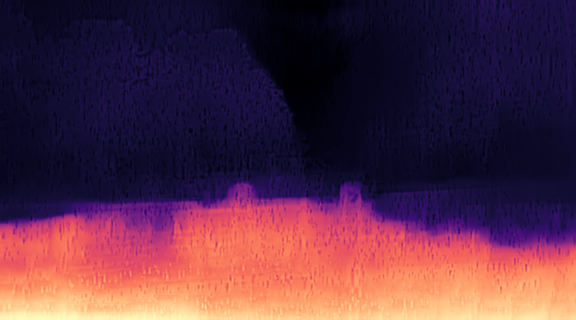
\includegraphics[width=0.191\linewidth]{figures/results/hybrid/monodepth2/100mm/011.png} & 
  
\includegraphics[width=0.191\linewidth]{figures/results/hybrid/monodepth2/200mm/011.png} \\
	
  & Clear weather  & GAN only  & Moderate rain  & Heavy rain  & Shower rain \\
  &      &     & (50~mm/hr)     & (100~mm/hr)  & (200~mm/hr) \\
 \end{tabular}
 \caption{\textbf{Depth estimation on our GAN+PBR augmented nuScenes.} From left to right, the original image (clear), the GAN augmented image and three GAN+PBR images.}
 \label{fig:eval_depth_estim_detect_qualitative_hybrid}
\end{figure*}
